\section{Resultados}

\subsection{Análise das métricas por linguagem de programação}
\begin{frame}{Análise das métricas por linguagem de programação}
    \begin{itemize}
        \item Potência média
        \item Memória máxima média
        \item Tempo médio por execução
        \item Temperatura média da CPU
    \end{itemize}
\end{frame}

\begin{frame}{Consumo em Joules por problema}
    \begin{figure}
        \centering
        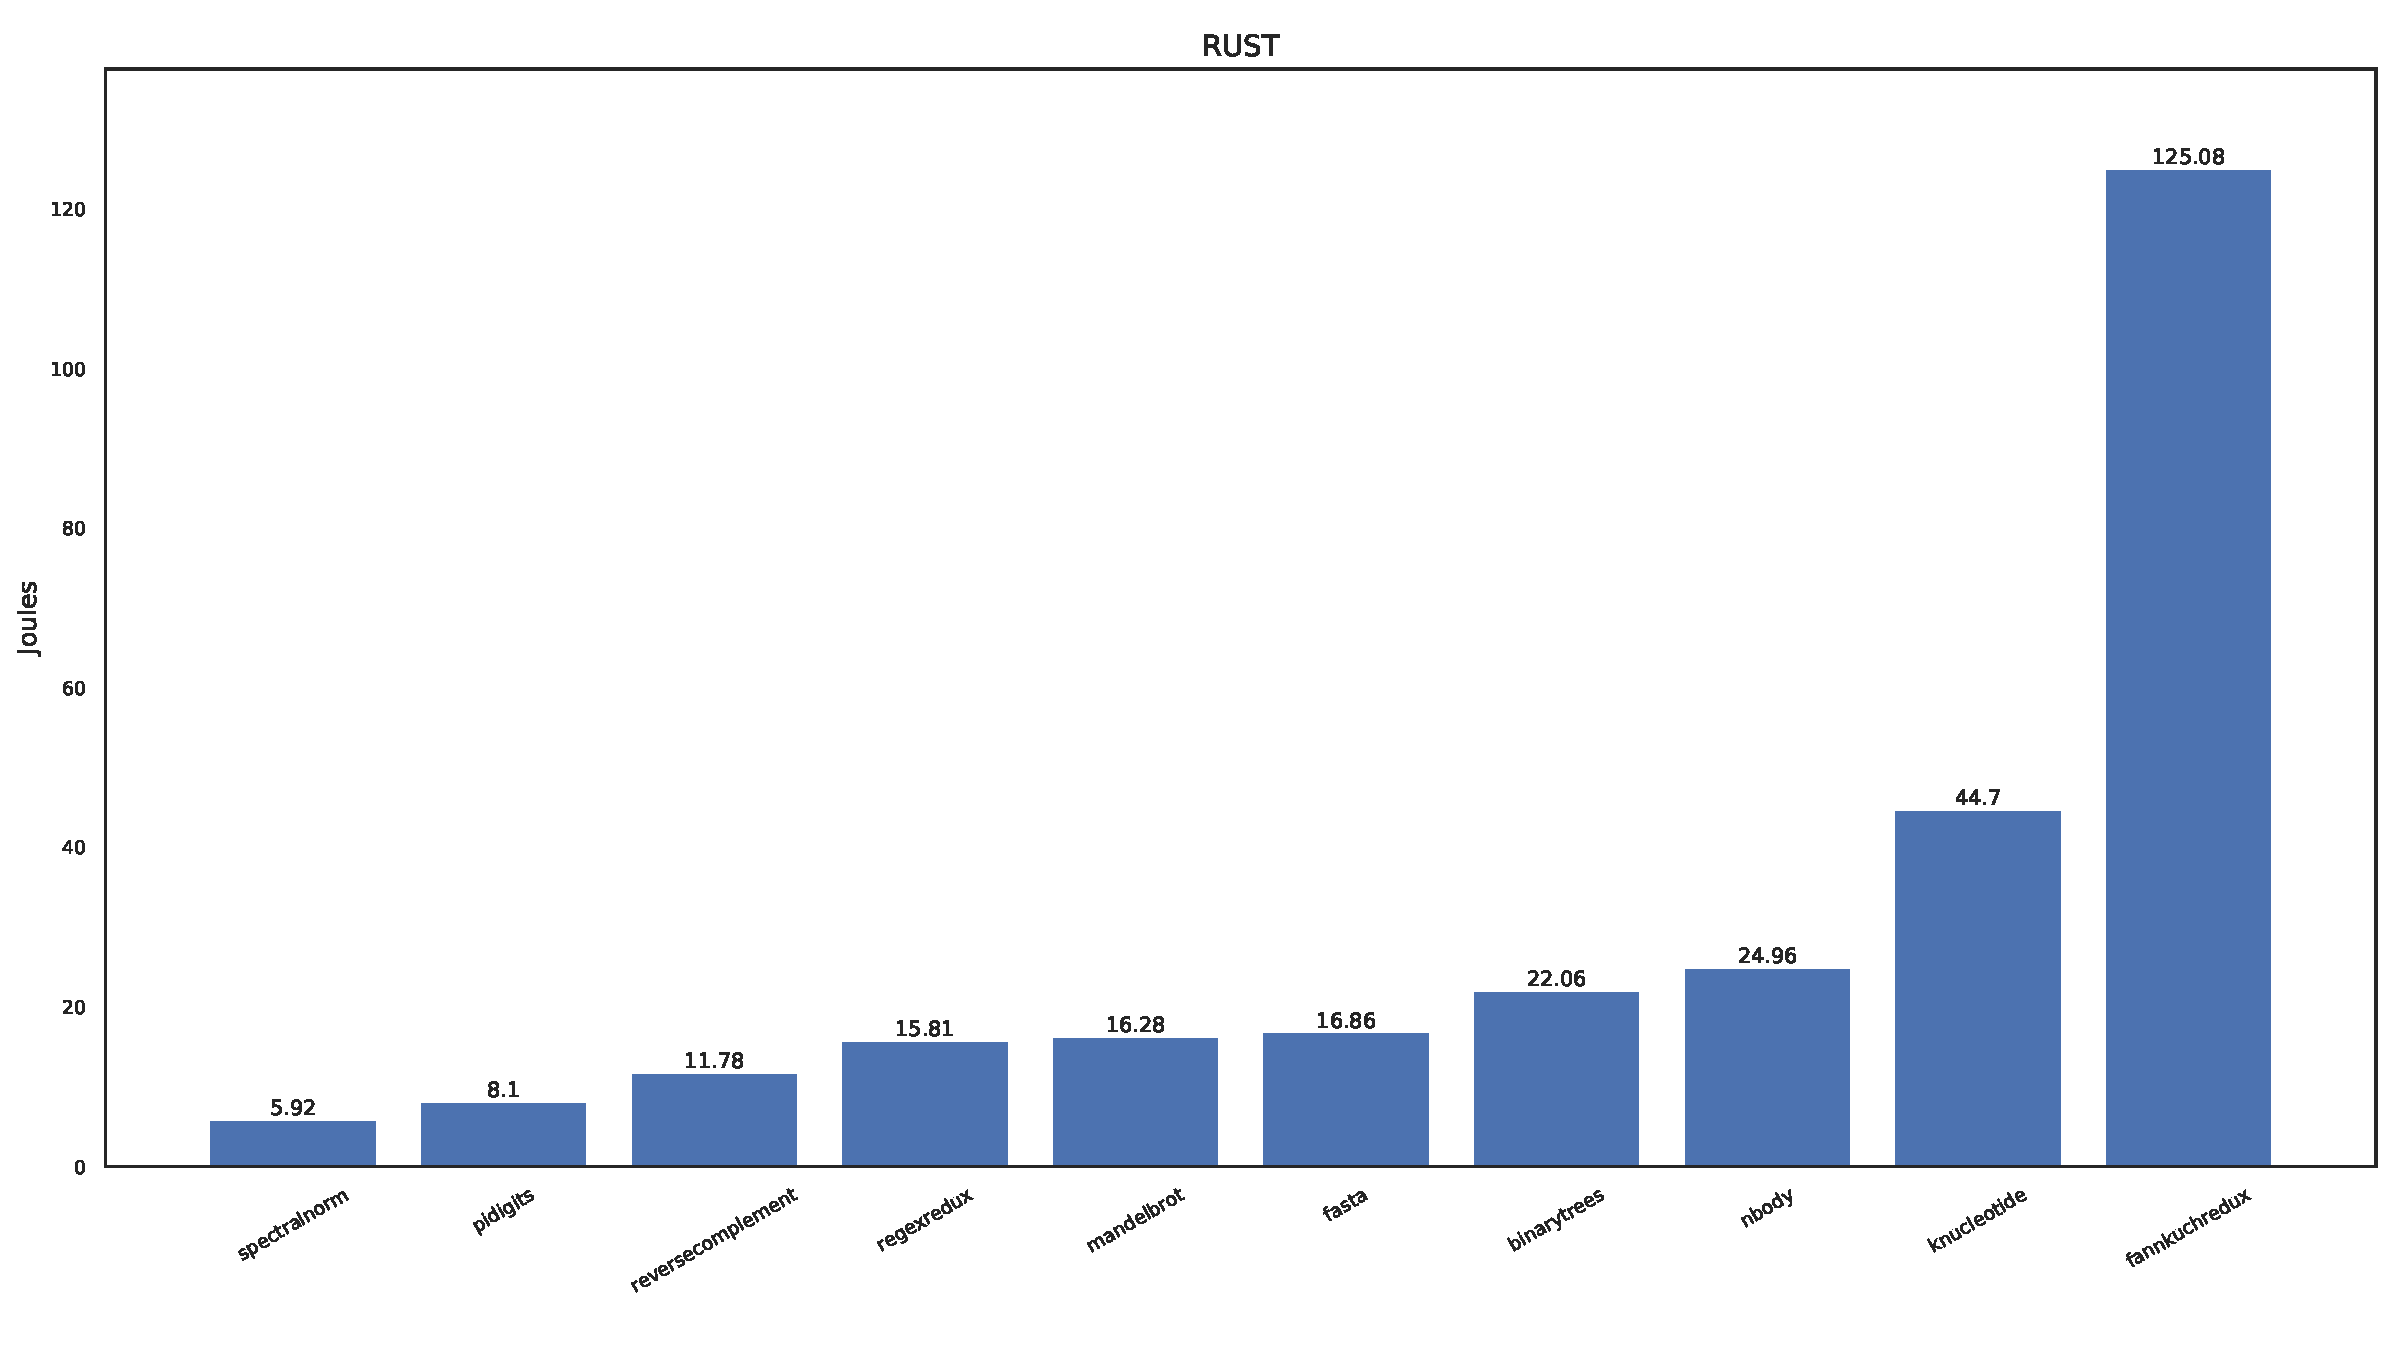
\includegraphics[width=0.85\linewidth]{images/rust-1.pdf}
        %\caption{Intel RAPL Power Domains. Fonte: Khan at al 2018 \cite{khan2018IntelRapl}}
        \label{fig:powerDomains2c3s4}
    \end{figure}
\end{frame}

\begin{frame}{Potência, memória, tempo e temperatura}
    \begin{figure}
        \centering
        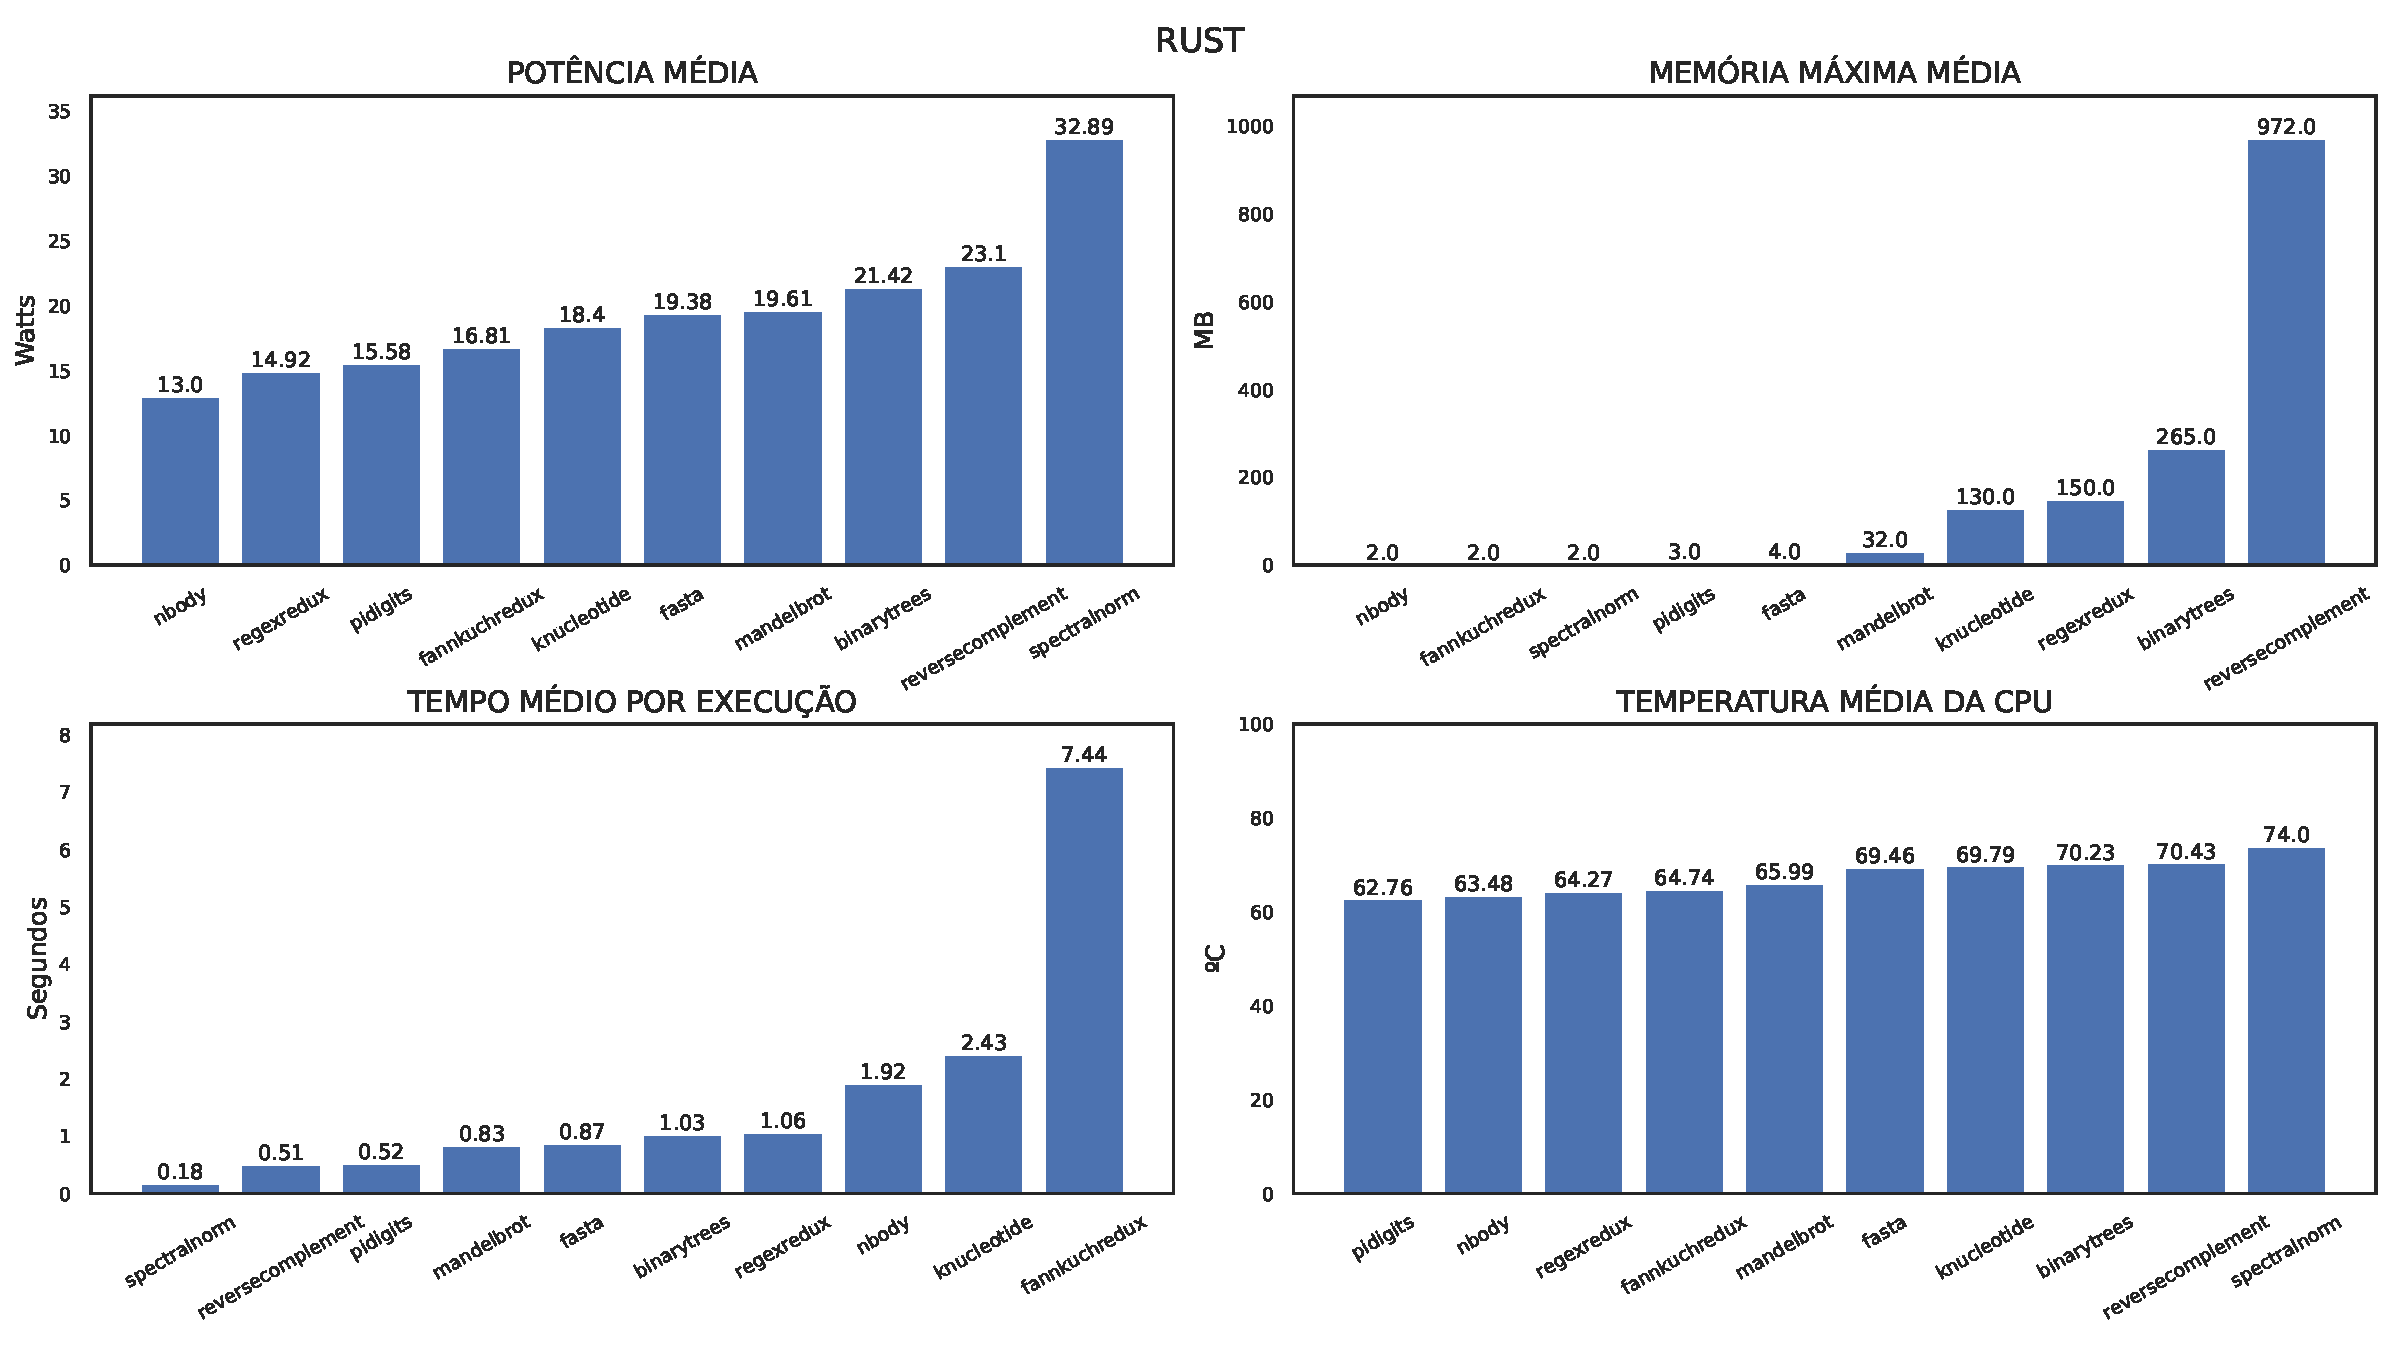
\includegraphics[width=0.85\linewidth]{images/rust-2.pdf}
        %\caption{Intel RAPL Power Domains. Fonte: Khan at al 2018 \cite{khan2018IntelRapl}}
        \label{fig:powerDomainsrusat2c3s4}
    \end{figure}
\end{frame}

\subsection{Eficiência energética}
\begin{frame}{Energia por execução}
    \begin{figure}
        \centering
        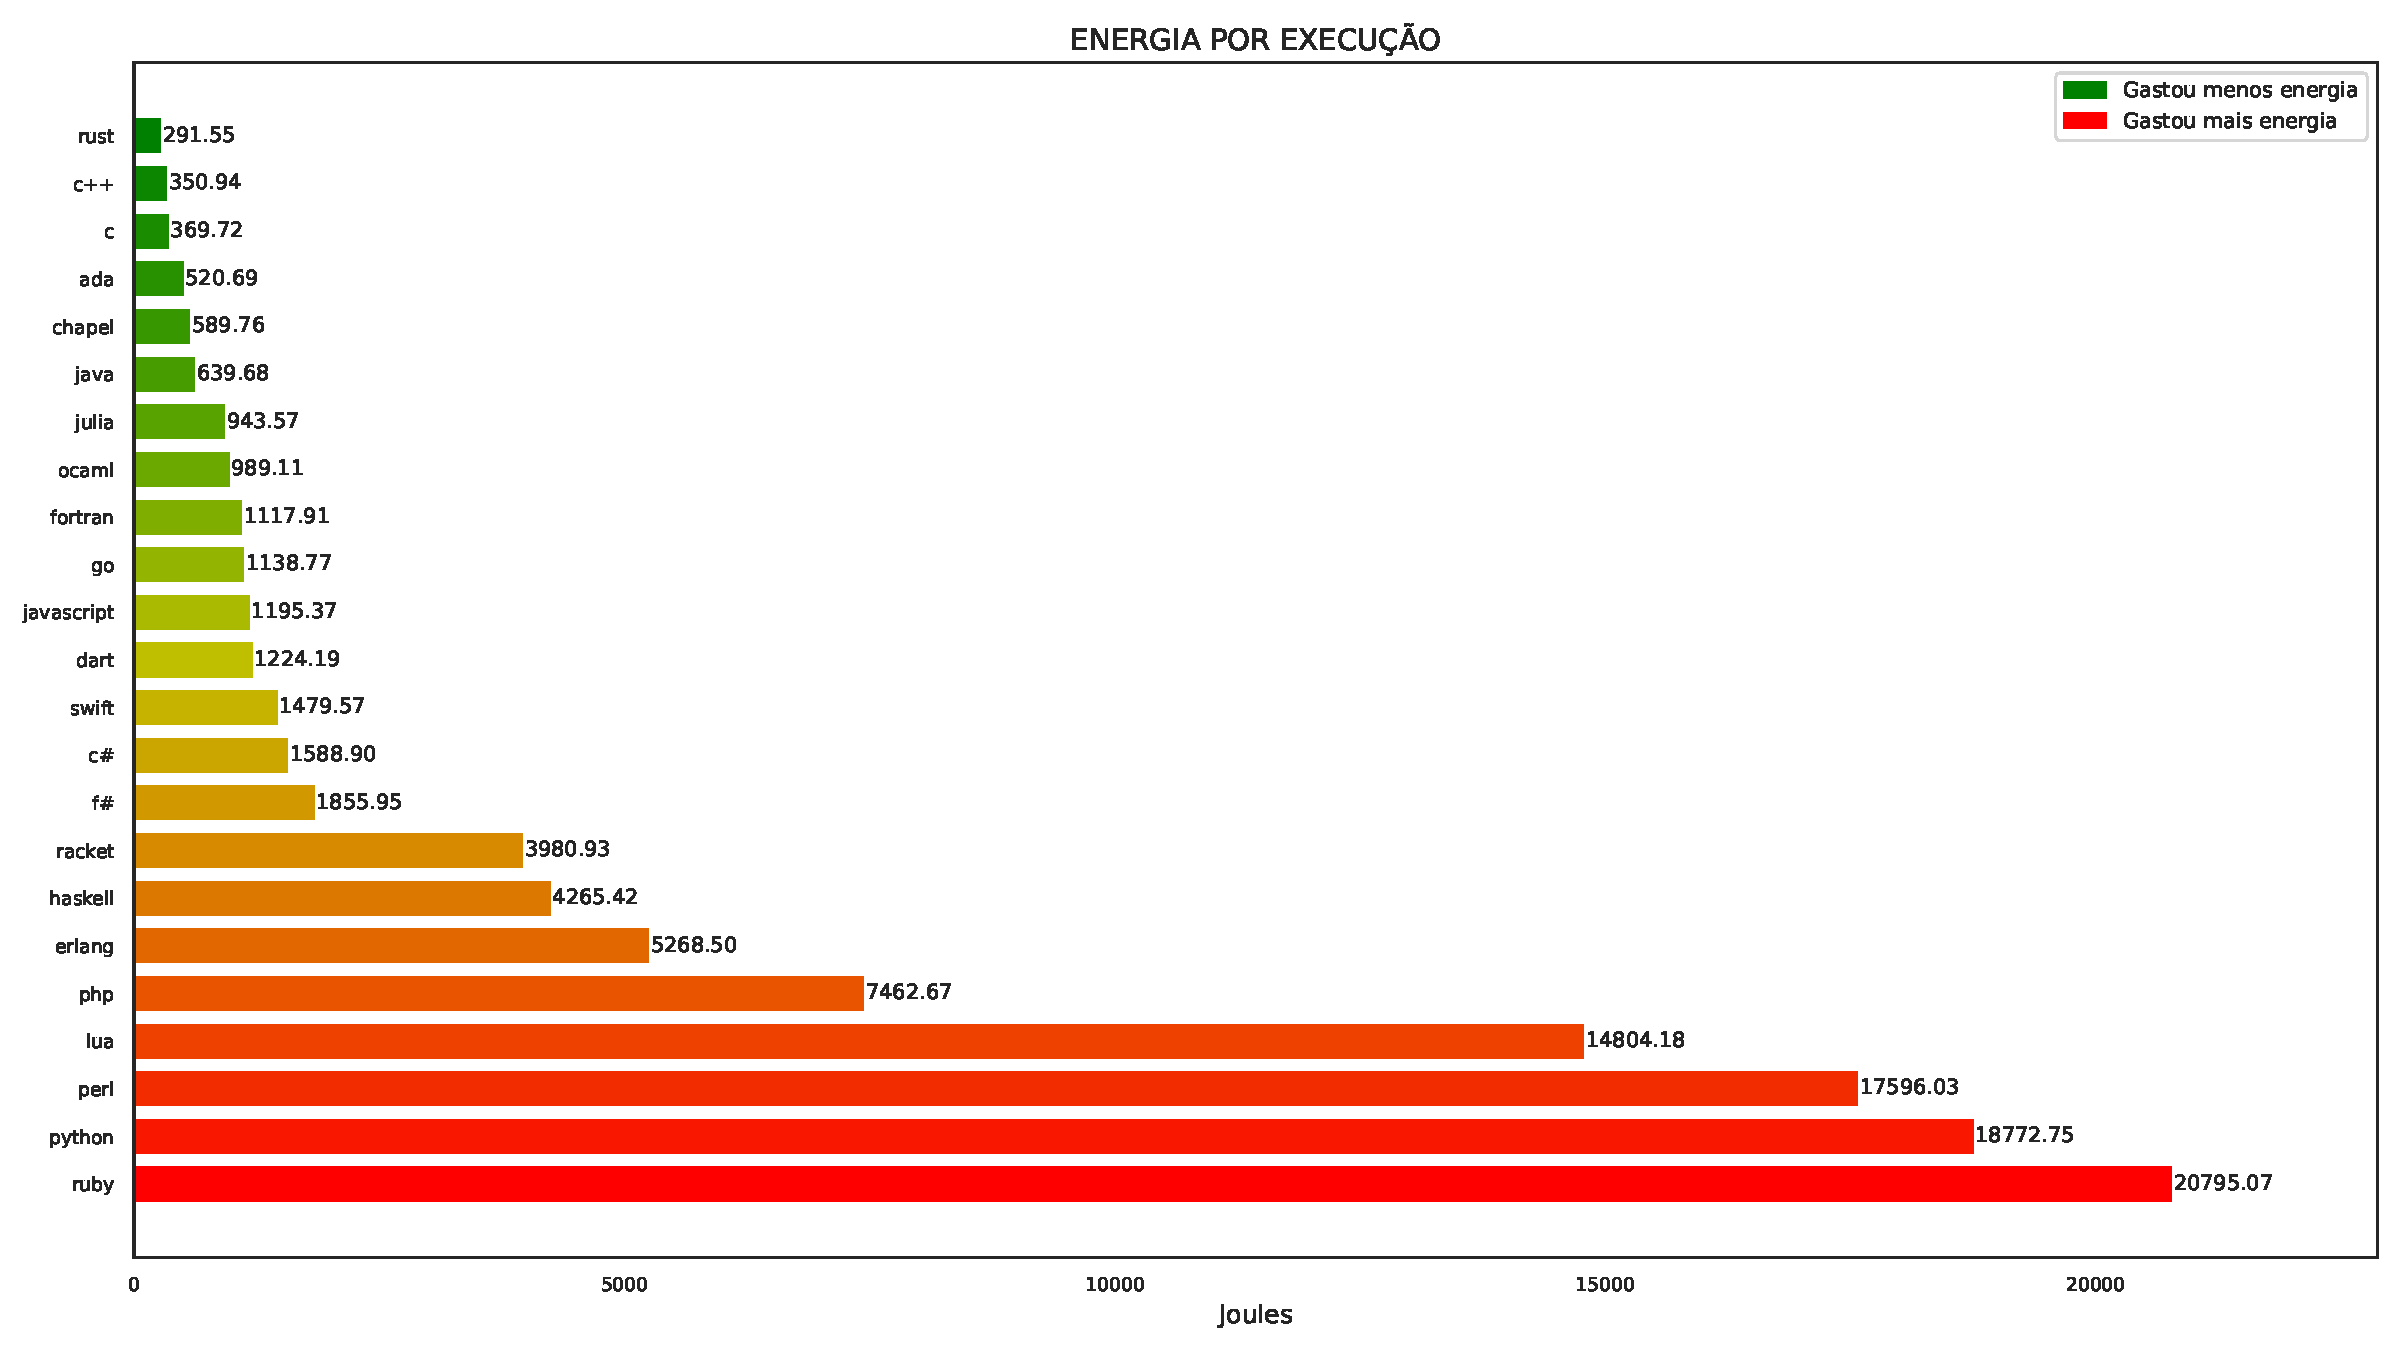
\includegraphics[width=0.85\linewidth]{images/energia_por_execucao.pdf}
        \caption{Intel RAPL Power Domains. Fonte: Khan at al 2018 \cite{khan2018IntelRapl}}
    \end{figure}
\end{frame}

\begin{frame}{Eficiência energética}
    \begin{figure}
        \centering
        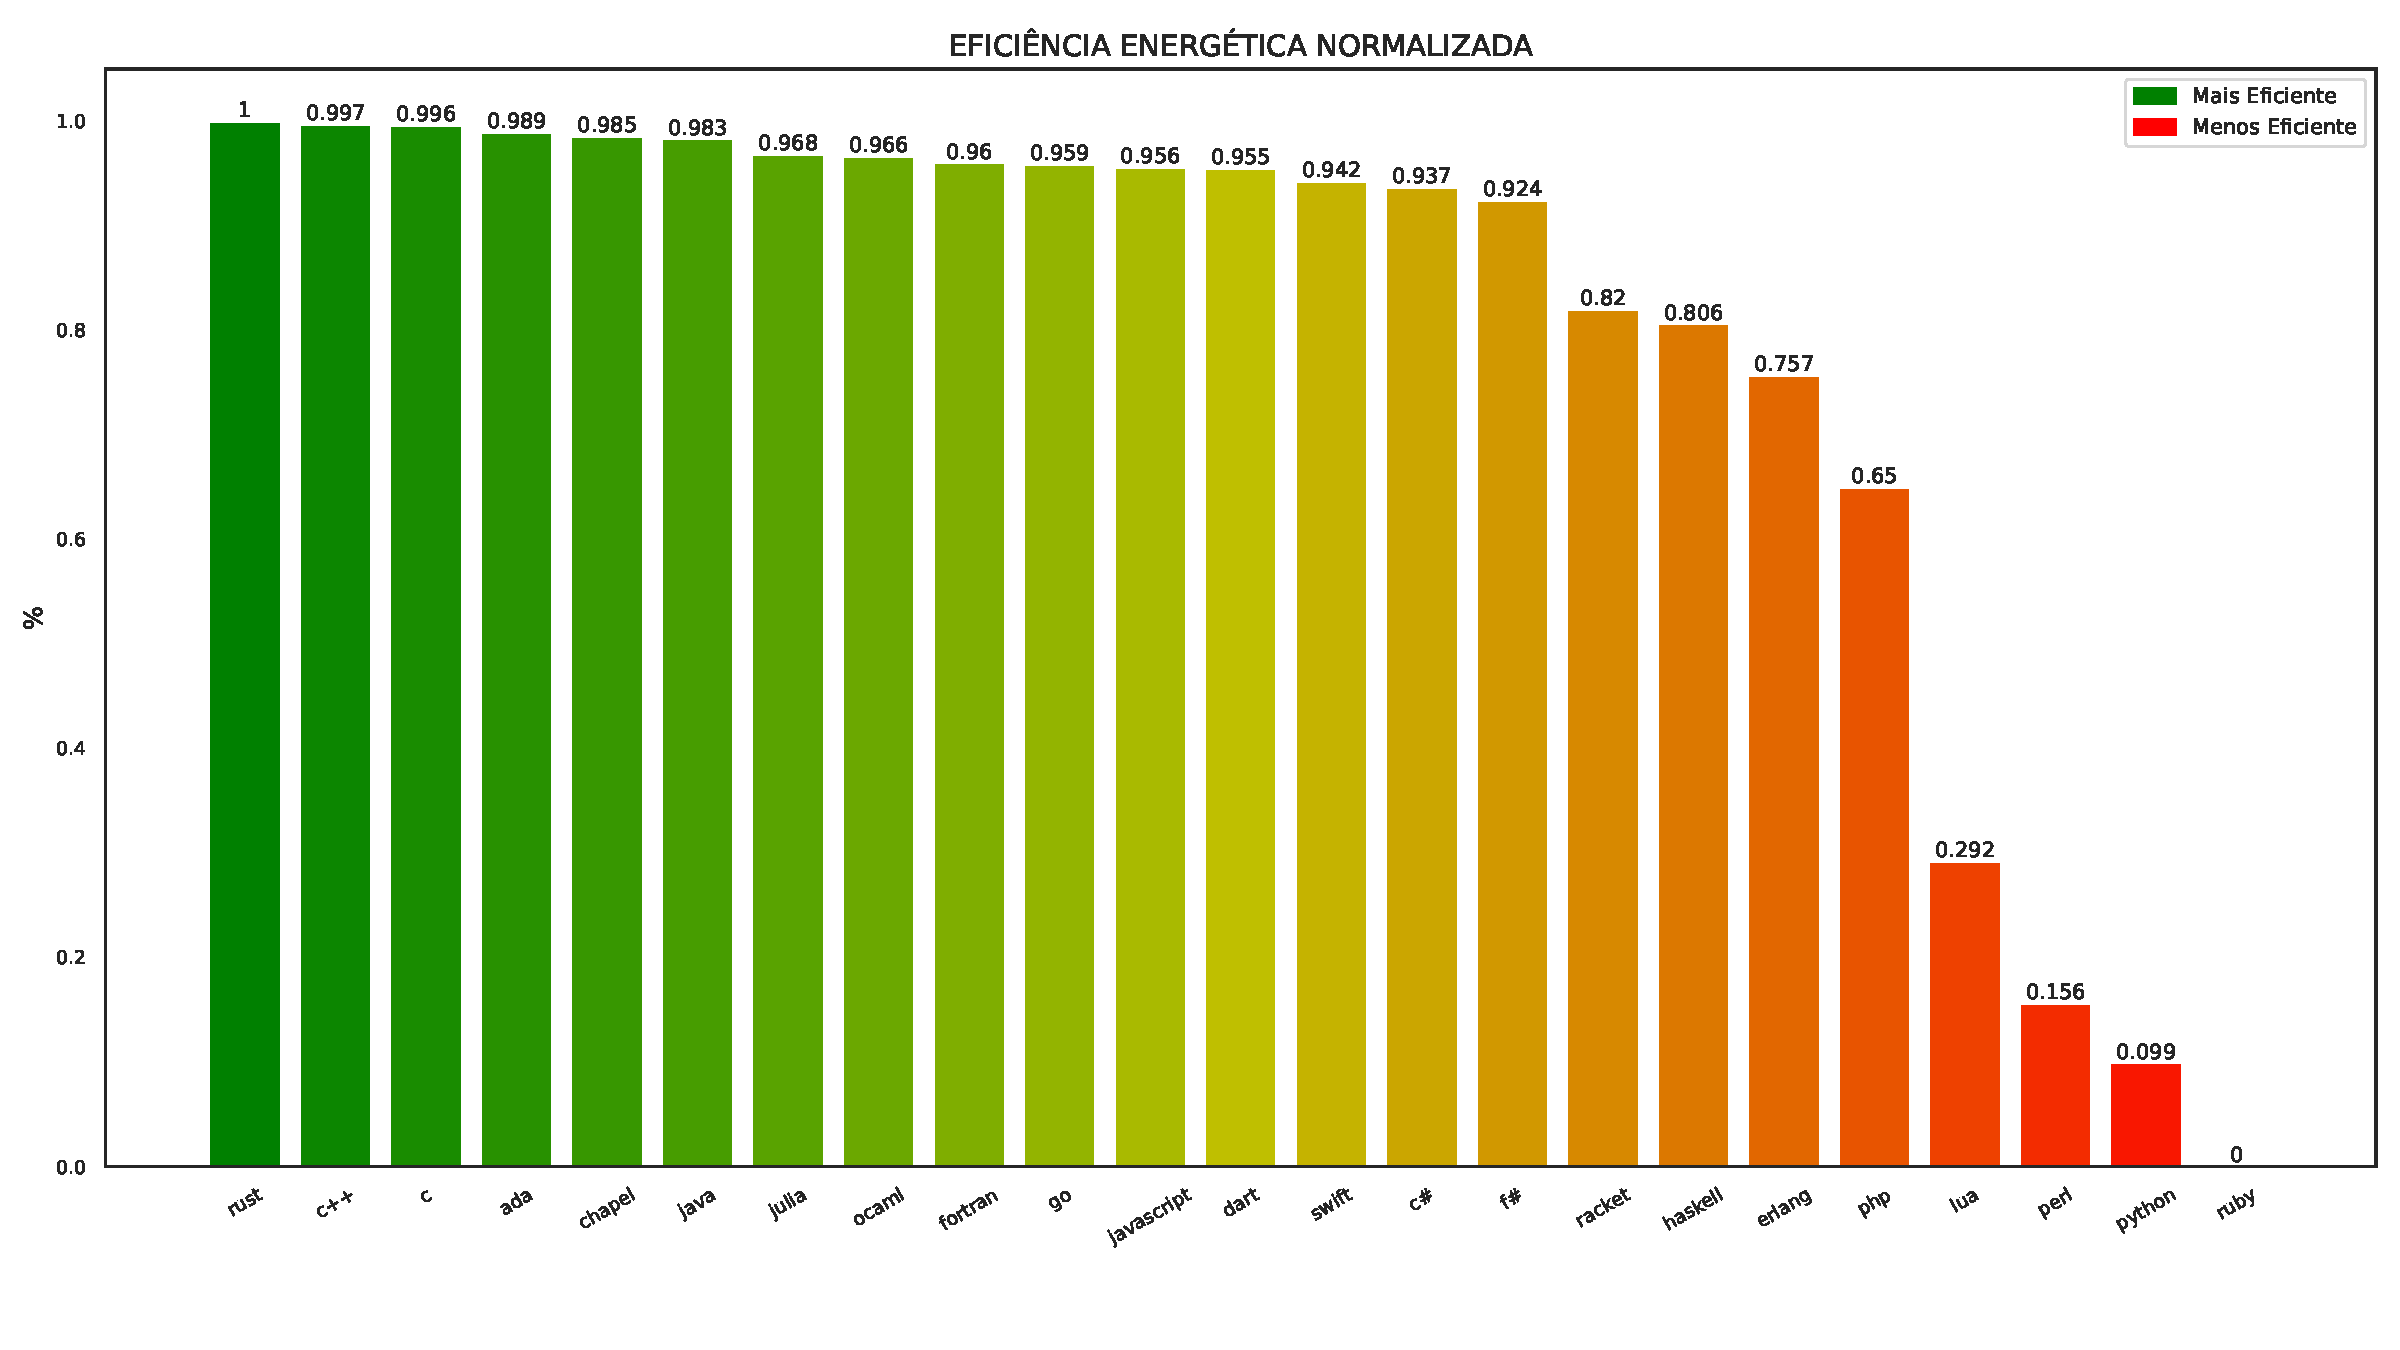
\includegraphics[width=0.85\linewidth]{images/eficiencia_energetica.pdf}
        %\caption{Intel RAPL Power Domains. Fonte: Khan at al 2018 \cite{khan2018IntelRapl}}
    \end{figure}
\end{frame}

\subsection{Análise do custo financeiro}
\begin{frame}{Análise do custo financeiro por 1000 execuções}
    \begin{itemize}
        \item A tarifa média considerada foi de 0.73 centavos por kWh
        \item Utilizamos o consumo total em Joules e convertemos para kWh
        \item Multiplicamos o consumo total em kWh por 1000 execuções
    \end{itemize}
 

    \begin{equation}
        \text{{Consumo em kWh}} = \frac{{\text{{Consumo em Joules}}}}{{3.600.000}}
    \end{equation}
\end{frame}

\begin{frame}{Linguagens de programação}
    \centering
    \begin{table}[!hp]
      %\caption{Linguagens de programação}
      %\label{tbl:custo}
      \centering
      %\rowcolors{2}{lightgray!30}{white}
      \fontsize{6}{7}\selectfont
      \begin{tabular}{l|l|l|l|l}
        \toprule
        \textbf{Linguagem} & \textbf{Joules} & \textbf{kWh} & \textbf{kWh por mil execuções} & \textbf{Custo por mil execuções (R\$)} \\
        \toprule
        Rust & 291,55 & 0,000081 & 0,081 & 0,05913 \\
        \hline
        C++ & 350,94 & 0,000098 & 0,098 & 0,07154 \\
        \hline
        C & 369,72 & 0,000103 & 0,103 & 0,07519 \\
        \hline
        Ada & 520,69 & 0,000145 & 0,145 & 0,10585 \\
        \hline
        Chapel & 589,76 & 0,000164 & 0,164 & 0,11972 \\
        \hline
        Java & 639,68 & 0,000178 & 0,178 & 0,12994 \\
        \hline
        Julia &  943,57 & 0,000262 & 0,262 & 0,19126 \\
        \hline
        Ocaml & 989,11 & 0,000275 & 0,275 & 0,20075 \\
        \hline
        Fortran & 1117,91 & 0,000310 & 0,310 & 0,2263 \\
        \hline
        Go & 1138,77 & 0,000316 & 0,316 & 0,23068 \\
        \hline
        Javascript & 1195,37 & 0,000332 & 0,332 & 0,24236 \\
        \hline
        Dart & 1224,19 & 0,000340 & 0,340 & 0,2482 \\
        \hline
        Swift & 1479,57 & 0,000411 & 0,411 & 0,30003 \\
        \hline
        C\# & 1588,90 & 0,000441 & 0,441 & 0,32193 \\
        \hline
        F\# & 1855,95 & 0,000516 & 0,516 & 0,37668 \\
        \hline
        Racket & 3980,93 & 0,001106 & 1,106 & 0,80738 \\
        \hline
        Haskell & 4265,42 & 0,001184 & 1,184 & 0,86432 \\
        \hline
        Erlang & 5268,50 & 0,001463 & 1,463 & 1,06799 \\
        \hline
        PHP & 7462,67 & 0,002073 & 2,073 & 1,51329 \\
        \hline
        Lua & 14804,18 & 0,004112 & 4,112 & 3,00176 \\
        \hline
        Perl & 17596,03 & 0,004888 & 4,888 & 3,56824 \\
        \hline
        Python & 18772,75 & 0,005214 & 5,214 & 3,80622 \\
        \hline
        Ruby & 20795,07 & 0,005777 & 5,777 & 4,21721 \\
        \bottomrule
      \end{tabular}
    \end{table}
\end{frame}
